\section{Approximate Abstraction on Example Domains}

%Explanation of what abstraction is used
We compare the number of states in the abstract MDP to different values of $\epsilon$, as well as the value difference between the optimal policy in the abstract MDP compared to the ground MDP. More specifically, we relate $\epsilon$ to:
\begin{equation}
|V^{\pi_G^*}(s_{init}) - V^{\pi_A^*}(s_{init})|
\end{equation}
For different values of $\epsilon$.

\dnote{Also put in a note that we're using a uniform weighting scheme}
\enote{Also put in a note how we're randomly choosing a Q*}
%Explain plots
Here we discuss the results shown in states blah blah \dnote{Description of this section}.

%Discuss results
Our empirical results corroborate our thesis -- that approximate state abstractions can form the basis of learnable and useful state aggregation criteria. In both NChain and Minefield, we observe that despite increasing $\epsilon$ to reduce the number of states which must be planned over, optimal behavior is either fully maintained (NChain) or optimal behavior is very nearly maintained (Minefield). Similarly for Taxi and $\epsilon$ between $.02$ and $.025$ we observe a reduction in the number of states that must be planned over while value is fully maintained. After $.025$, increased reduction in state space size comes at a cost of value. Lastly, as $\epsilon$ is increased Random smoothly reduces the number of abstract states which must be planned over with a corresponding cost in the value of the derived policy.

Our experimental results also demonstrate a noteworthy contrast between approximate state abstraction on goal-based \acp{MDP} and random \acp{MDP}. Taxi exhibits relative stability in state space size and behavior for epsilon up to $.02$ until both precipitously fall off. We attribute the sudden fall off in number of abstract states and value of the derived policy in Taxi to its goal-based nature; once certain information critical for optimal behavior is lost in the state aggregation, solving the goal -- and so acquiring any reward -- is rendered entirely unattainable. Conversely, in Random a great deal of near-optimal policies are available to the agent. Thus, even the information for optimal behavior is lost with an increase in $\epsilon$ there are a great deal of near-optimal policies available to the agent which are not lost in the state aggregation.

% Figure: Epsilon vs. #States and Epsilon vs Abstract Pol. Value for all four sample domains.
\begin{figure}
\centering

\subfigure[NChain]{
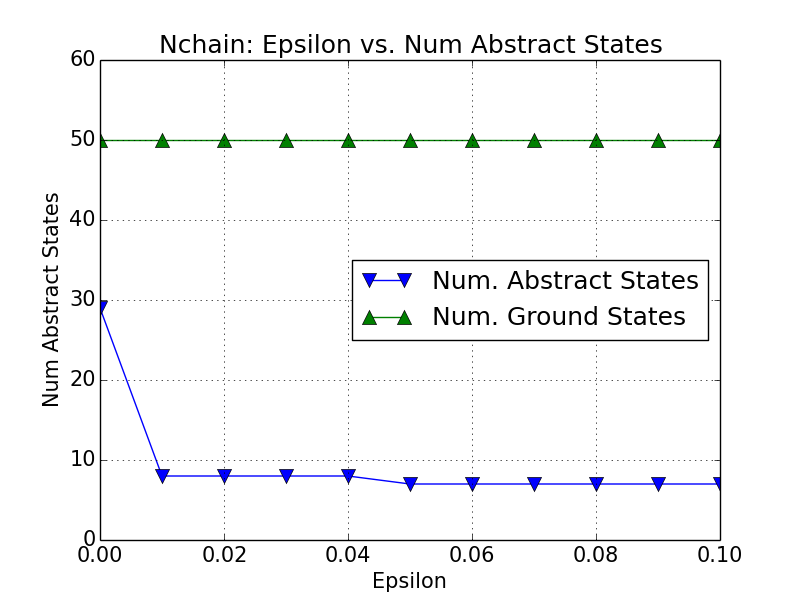
\includegraphics[width=0.46\columnwidth]{figures/nchain_epsilon_vs_num_abstract_states.png}
}
\subfigure[NChain]{
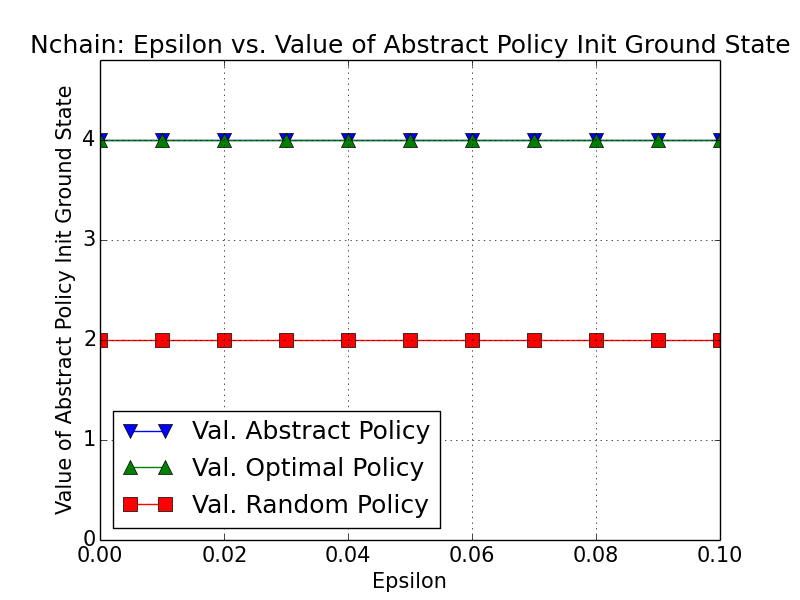
\includegraphics[width=0.46\columnwidth]{figures/nchain_epsilon_vs_value_of_abstract_policy_init_ground_state.png}
}

\subfigure[Minefield]{
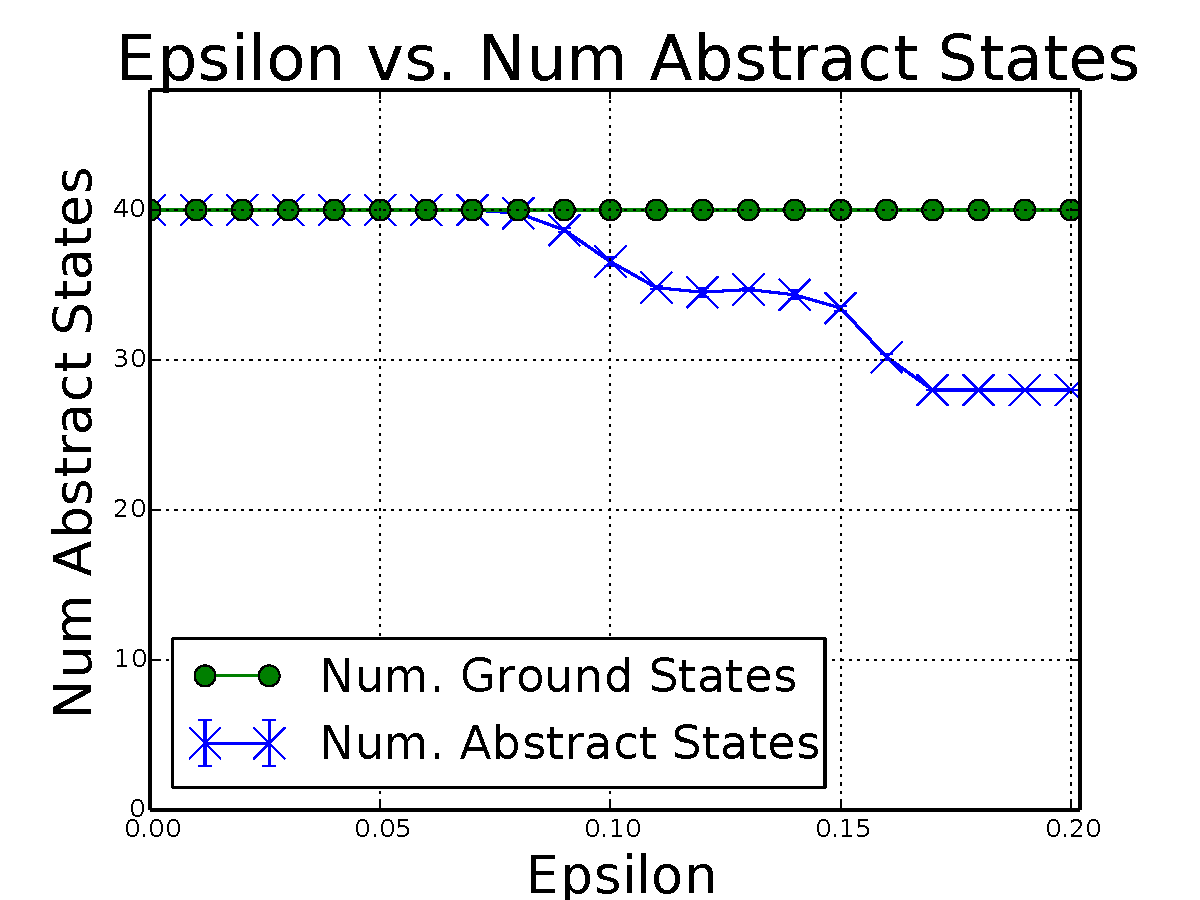
\includegraphics[width=0.46\columnwidth]{figures/minefield_epsilon_vs_num_abstract_states.pdf}
}
\subfigure[Minefield]{
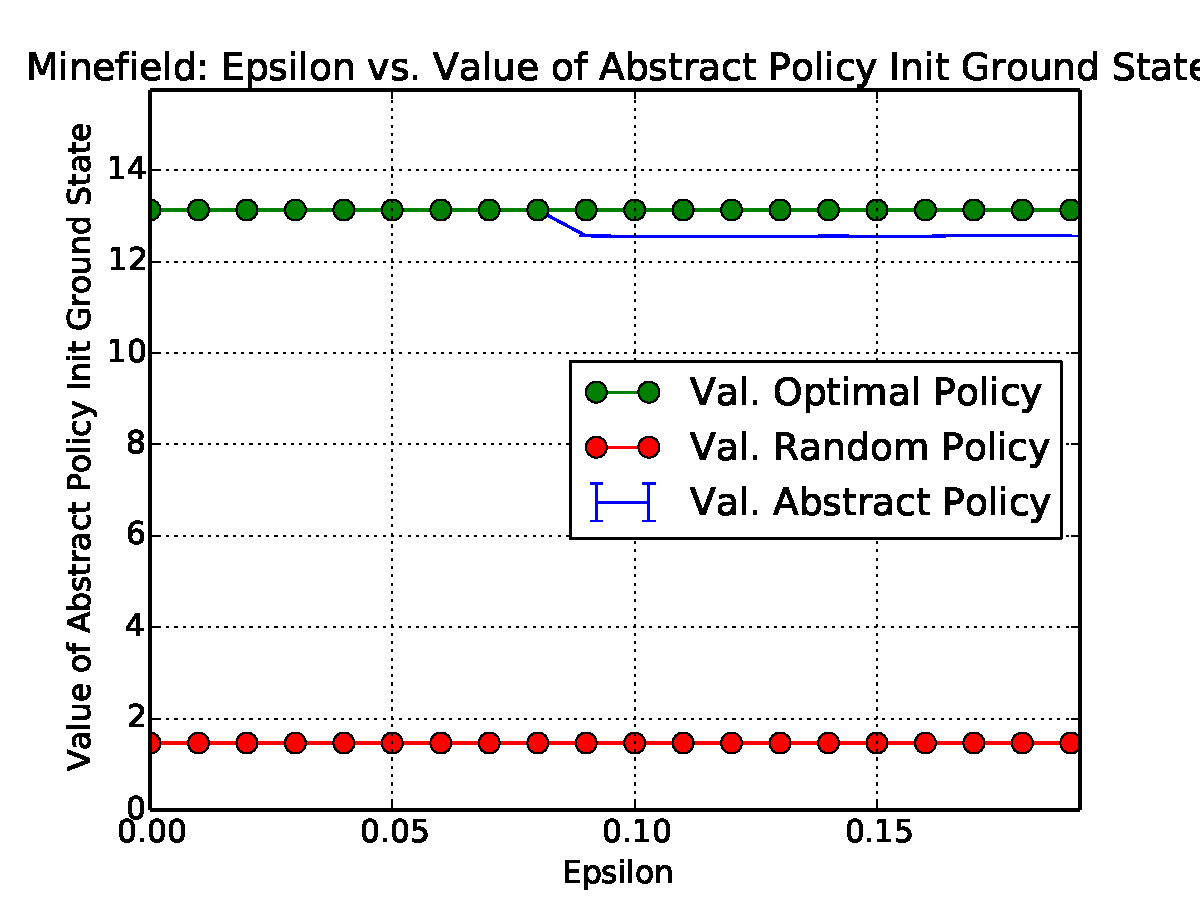
\includegraphics[width=0.46\columnwidth]{figures/minefield_epsilon_vs_value_of_abstract_policy_init_ground_state.pdf}
}

\subfigure[Taxi]{
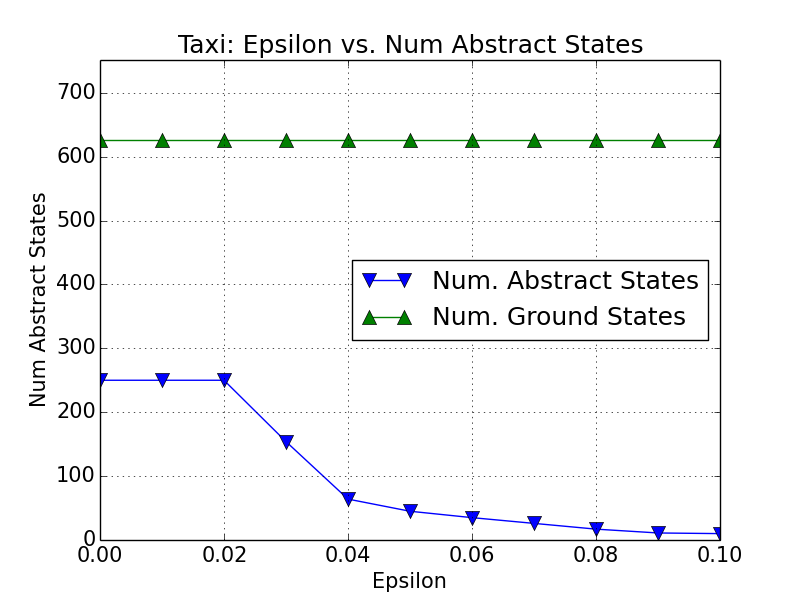
\includegraphics[width=0.46\columnwidth]{figures/taxi_epsilon_vs_num_abstract_states.png}
}
\subfigure[Taxi]{
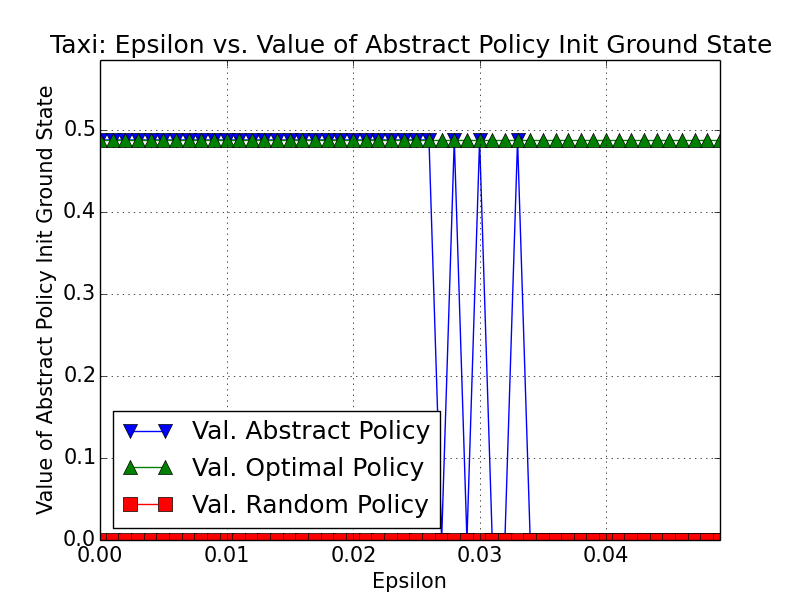
\includegraphics[width=0.46\columnwidth]{figures/taxi_epsilon_vs_value_of_abstract_policy_init_ground_state.png}
}

\subfigure[Random]{
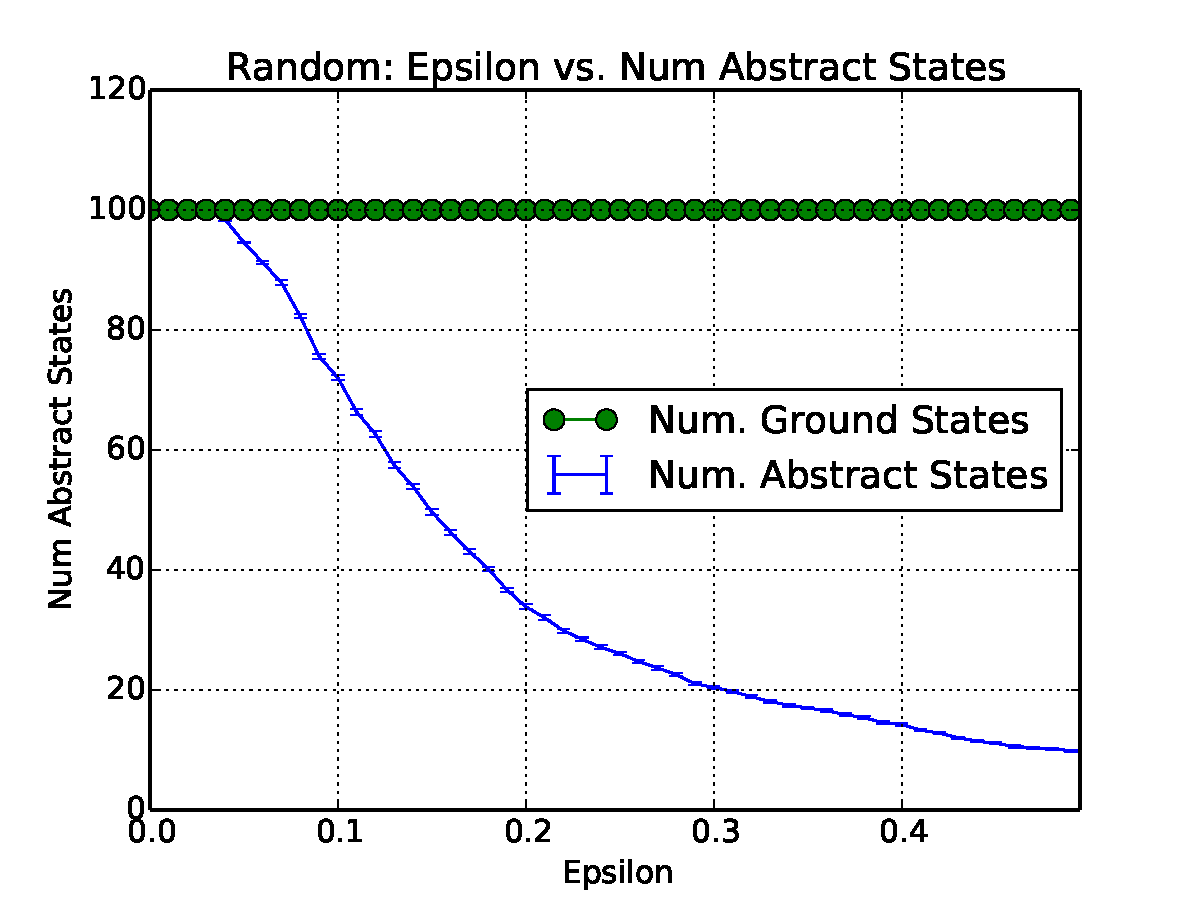
\includegraphics[width=0.46\columnwidth]{figures/random_epsilon_vs_num_abstract_states.pdf}
}
\subfigure[Random]{
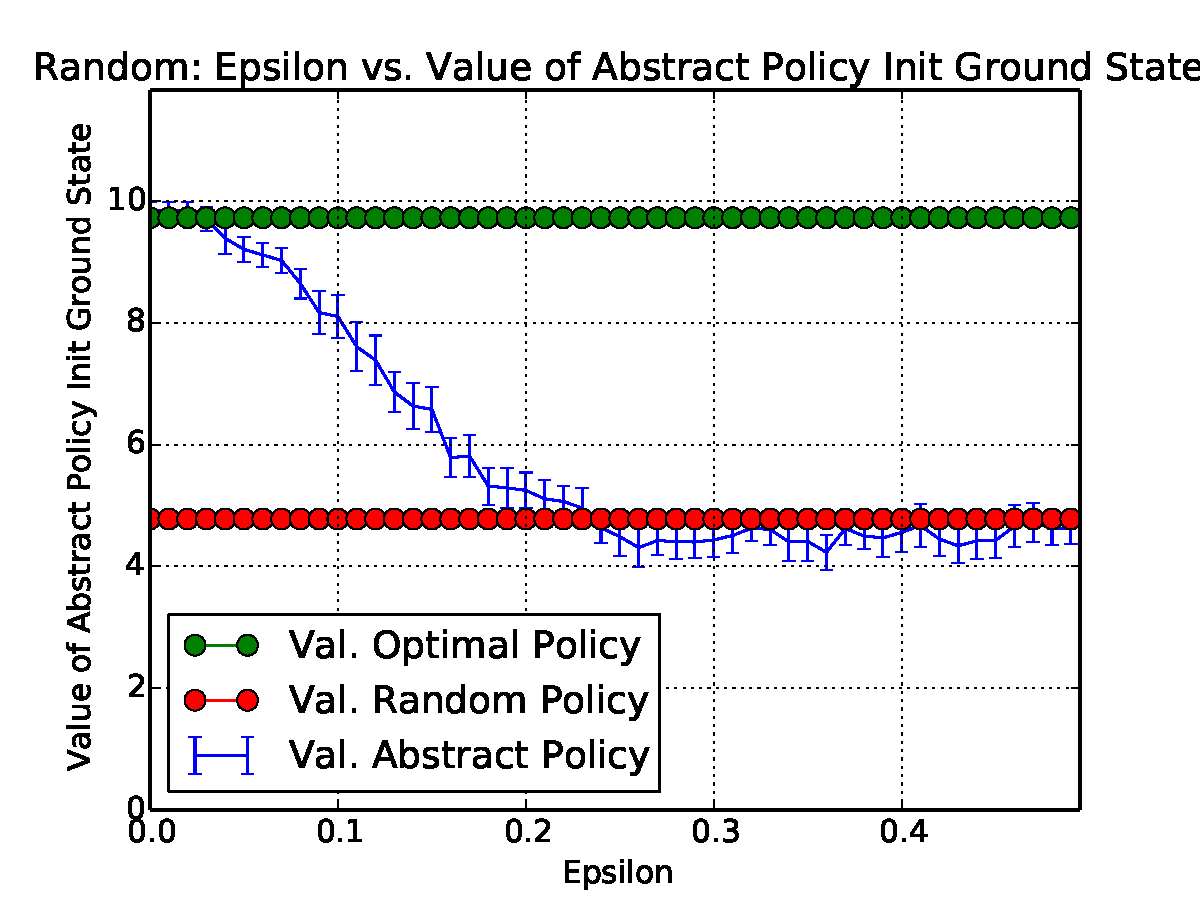
\includegraphics[width=0.46\columnwidth]{figures/random_epsilon_vs_value_of_abstract_policy_init_ground_state.pdf}
}

\label{fig:main_empirical_results}
\caption{$\epsilon$ vs. Num States and $\epsilon$ vs. Abstract Policy Value}
\end{figure} 
